A lot of work has been done in this field, resulting in many different prefetching heuristics. They
range from the very simple sequential ones, that simply fetches the address after the current one,
to more complex ones that tries to find patterns and use dynamically gathered statistics to guide
them \cite{prefetch_range}.

\subsection{Reference Prediction Tables}
Reference Prediction Tables (RPT) is a prefetching technique which uses a large table to store information indexed by the program counter of the load. It calculates the delta for each miss, but the prefetching is only done after a certain amount of misses with the delta has occured.

\subsection{Program Counter/Delta Correlation Prefetching}
Program Counter/Delta Correlation Prefetching (PC/DC) is a prefetching method using a Global History Buffer (GHB). It uses buffered delta calculations to search for stride patterns. If a pattern is found, it is used to start prefetching.

\subsection{Delta Correlation Prediction Tables} 
Delta Correlation Prediction Tables combines RPT and PC/DC \cite{dcpt}. A large table is indexed by
the program counter and Fig.~\ref{fig:dcpt_entry} shows an entry in the table.
\begin{figure}[h]
	\begin{center}
		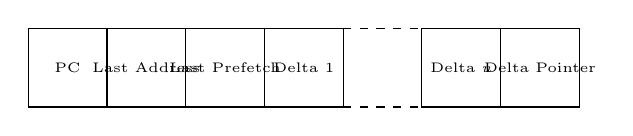
\begin{tikzpicture}
			\draw (0,0) rectangle (1,1);
			\draw (1,0) rectangle (2,1);
			\draw (2,0) rectangle (3,1);
			\draw (3,0) rectangle (4,1);
			\draw[dashed] (4,0) -- (5,0);
			\draw[dashed] (4,1) -- (5,1);
			\draw (5,0) rectangle (6,1);
			\draw (6,0) rectangle (7,1);

			\draw (0.5,0.5) node {\tiny PC};
			\draw (1.5,0.5) node {\tiny Last Address};	
			\draw (2.5,0.5) node {\tiny Last Prefetch};
			\draw (3.5,0.5) node {\tiny Delta 1};
			\draw (5.5,0.5) node {\tiny Delta \emph{n}};
			\draw (6.5,0.5) node {\tiny Delta Pointer};
		\end{tikzpicture}
	\end{center}
	\caption{DCPT entry\label{fig:dcpt_entry}}
\end{figure}
The PC entry contains the program counter of the load instruction. Last address contains the load
address. The delta fields contains the calculated delta values for this load instruction. These
delta fields works as a circular buffer, where the delta pointer field points to the head of the
buffer. Last prefetch stores the last prefetch address.






